\documentclass[%
reprint,
superscriptaddress,
%groupedaddress,
%unsortedaddress,
%runinaddress,
%frontmatterverbose, 
%=preprint,
showpacs,
%preprintnumbers,
nofootinbib,
%nobibnotes,
bibnotes,amsmath,amssymb,aps,
%pra,
%prb, 
prc, 
%rmp,
%prstab,  
%prstper,
%floatfix,
]{revtex4-1}

\usepackage{graphicx,dblfloatfix,afterpage,caption}
\usepackage{dcolumn}
\usepackage{bm}
\usepackage[colorlinks=true,urlcolor=blue,citecolor=blue,linkcolor=blue]{hyperref}
\usepackage{color}
\usepackage{natbib}
\usepackage{float}
\usepackage{soul}
\usepackage{caption}

\usepackage{listings}
\usepackage{color}

\definecolor{dkgreen}{rgb}{0,0.6,0}
\definecolor{gray}{rgb}{0.5,0.5,0.5}
\definecolor{mauve}{rgb}{0.58,0,0.82}

\lstset{frame=tb,
	language=Java,
	aboveskip=3mm,
	belowskip=3mm,
	showstringspaces=false,
	columns=flexible,
	basicstyle={\small\ttfamily},
	numbers=none,
	numberstyle=\tiny\color{gray},
	keywordstyle=\color{blue},
	commentstyle=\color{dkgreen},
	stringstyle=\color{mauve},
	breaklines=true,
	breakatwhitespace=true,
	tabsize=3
}




\begin{document}
	\title{Project 1}
	\author{Eric Aboud}
	\affiliation{Department of Physics and Astronomy, Michigan State University, East Lansing, MI 48823}
	\author{Parker Brue}
	\affiliation{Department of Physics and Astronomy, Michigan State University, East Lansing, MI 48823}
	\begin{abstract}
	We present an algorithm that allows us to solve the Schr$\ddot{\textrm{o}}$dinger equation for electron-electron interactions.  Using Jacobi rotation methods, we are able to solve for the eigenvalues for a known potential equation.  Using inherent eignenvalue solvers, we are able to verify the eigenvalues obtained through the Jacobi rotation methods.  Comparisons between potential strengths provide insight on electron-electron interactions.
	\end{abstract}
	\maketitle
	
	
	\section{Introduction}
	
	One of the simplest cases of the Schr$\ddot{\textrm{o}}$dinger equation comes from electron-electron interactions within a three-dimensional harmonic oscillator.  To further simplify the problem, we can first solve for a case with no Coulomb interactions.  Using multiple eigenvalue solvers (Jacobi rotations and built-in solvers) we are able to determine the eigenvalues resulting from a given Schr$\ddot{\textrm{o}}$dinger equation.  Analysis of the results provide insight on the effectiveness of the eigenvalue solvers.
	
	
	\section{Theory, algorithms and methods}
\subsection{Schroedinger's Equation for two electrons in a three-dimesnional harmonic oscillator well, noninteracting}	
The radial part of Schroedinger's equation for one electron reads

\begin{equation*}
	-\frac{\hbar^2}{2 m} \left ( \frac{1}{r^2} \frac{d}{dr} r^2
	\frac{d}{dr} - \frac{l (l + 1)}{r^2} \right )R(r) 
	+ V(r) R(r) = E R(r).
\end{equation*}
$V(r)$ is the harmonic oscillator potential $(1/2)kr^2$ with
$k=m\omega^2$ and $E$ is
the energy of the harmonic oscillator in three dimensions.
The oscillator frequency is $\omega$ and the energies are

\begin{equation*}
	E_{nl}=  \hbar \omega \left(2n+l+\frac{3}{2}\right),
\end{equation*}
with $n=0,1,2,\dots$ and $l=0,1,2,\dots$.

Due to the transformation to spherical coordinates
$r\in [0,\infty)$.  
The quantum number
$l$ is the orbital momentum of the electron.  
% 
Substituting $R(r) = (1/r) u(r)$:
% 

\begin{equation*}
	-\frac{\hbar^2}{2 m} \frac{d^2}{dr^2} u(r) 
	+ \left ( V(r) + \frac{l (l + 1)}{r^2}\frac{\hbar^2}{2 m}
	\right ) u(r)  = E u(r) .
\end{equation*}
% 
boundary conditions are $u(0)=0$ and $u(\infty)=0$.

We introduced a dimensionless variable $\rho = (1/\alpha) r$
where $\alpha$ is a constant length:
% 

\begin{equation*}
	-\frac{\hbar^2}{2 m \alpha^2} \frac{d^2}{d\rho^2} u(\rho) 
	+ \left ( V(\rho) + \frac{l (l + 1)}{\rho^2}
	\frac{\hbar^2}{2 m\alpha^2} \right ) u(\rho)  = E u(\rho) .
\end{equation*}
% 
In stipulations of the project, $l=0$.
We inserted $V(\rho) = (1/2) k \alpha^2\rho^2$:

\begin{equation*}
	-\frac{\hbar^2}{2 m \alpha^2} \frac{d^2}{d\rho^2} u(\rho) 
	+ \frac{k}{2} \alpha^2\rho^2u(\rho)  = E u(\rho) .
\end{equation*}
And multiplied by $2m\alpha^2/\hbar^2$ on both sides:

\begin{equation*}
	-\frac{d^2}{d\rho^2} u(\rho) 
	+ \frac{mk}{\hbar^2} \alpha^4\rho^2u(\rho)  = \frac{2m\alpha^2}{\hbar^2}E u(\rho) .
\end{equation*}
The constant $\alpha$ was fixed after some algebra
so that


\begin{equation*}
	\alpha = \left(\frac{\hbar^2}{mk}\right)^{1/4}.
\end{equation*}
We defined

\begin{equation*}
	\lambda = \frac{2m\alpha^2}{\hbar^2}E,
\end{equation*}
so we were able to rewrite Schroedinger's equation as

\begin{equation*}
	-\frac{d^2}{d\rho^2} u(\rho) + \rho^2u(\rho)  = \lambda u(\rho) .
\end{equation*}

And evaluate it by considering the canon form of second derivative of a function $u$
\begin{equation}
u''=\frac{u(\rho+h) -2u(\rho) +u(\rho-h)}{h^2} +O(h^2),
\label{eq:diffoperation}
\end{equation}
where $h$ is defined as our step length.
Minimum and maximum values for the variable $\rho$ are
$\rho_{\mathrm{min}}=0$  and $\rho_{\mathrm{max}}$
(In our case, we set $\rho_{\mathrm{max}}$ to 7.0).

With a specified number of mesh points, $N$, 
$h$ can be defined as, with $\rho_{\mathrm{min}}=\rho_0$  and $\rho_{\mathrm{max}}=\rho_N$,

\begin{equation*}
	h=\frac{\rho_N-\rho_0 }{N}.
\end{equation*}
The value of $\rho$ at a point $i$ is then 
\[
\rho_i= \rho_0 + ih \hspace{1cm} i=1,2,\dots , N.
\]
Rewriting the Schroedinger equation for $\rho_i$ as

\[
-\frac{u_{i+1} -2u_i +u_{i-1}}{h^2}+\rho_i^2u_i=-\frac{u_{i+1} -2u_i +u_{i-1} }{h^2}+V_iu_i  = \lambda u_i,
\]
$V_i=\rho_i^2$ is the harmonic oscillator potential.

The diagonal matrix element is:
\begin{equation*}
	d_i=\frac{2}{h^2}+V_i,
\end{equation*}
and the non-diagonal matrix element is:
\begin{equation*}
	e_i=-\frac{1}{h^2}.
\end{equation*}
All non-diagonal matrix elements are equal, a constant.
The Schroedinger equation is now:

\begin{equation*}
	d_iu_i+e_{i-1}u_{i-1}+e_{i+1}u_{i+1}  = \lambda u_i,
\end{equation*}
$u_i$ is unknown. we rewrote this so we could solve for the matrix eigenvalues.
\begin{equation}
\begin{bmatrix}d_0 & e_0 & 0   & 0    & \dots  &0     & 0 \\
e_1 & d_1 & e_1 & 0    & \dots  &0     &0 \\
0   & e_2 & d_2 & e_2  &0       &\dots & 0\\
\dots  & \dots & \dots & \dots  &\dots      &\dots & \dots\\
0   & \dots & \dots & \dots  &\dots  e_{N-1}     &d_{N-1} & e_{N-1}\\
0   & \dots & \dots & \dots  &\dots       &e_{N} & d_{N}
\end{bmatrix}  \begin{bmatrix} u_{0} \\
u_{1} \\
\dots\\ \dots\\ \dots\\
u_{N}
\end{bmatrix}=\lambda \begin{bmatrix} u_{0} \\
u_{1} \\
\dots\\ \dots\\ \dots\\
u_{N}
\end{bmatrix}.  
\label{eq:sematrix}
\end{equation}
The values of $u$ at the two endpoints are known through the boundary conditions, allowing us to skip the involved rows and columns. we specified the matrix with our values for $d_i$ and $e_i$
\begin{equation}
\begin{bmatrix} \frac{2}{h^2}+V_1 & -\frac{1}{h^2} & 0        \\
-\frac{1}{h^2} & \frac{2}{h^2}+V_2 & -\frac{1}{h^2}     \\
0   & -\frac{1}{h^2} & \frac{2}{h^2}+V_{N-1} &     \\

\end{bmatrix}
\label{eq:matrixse} 
\end{equation}
This is the matrix we performed calculations on for the non interacting case

\subsection{Schroedinger's Equation for two electrons in a three-dimesnional harmonic oscillator well, interacting}	
We took the case of two electrons in a harmonic oscillator well, but
introduced an interaction via the repulsive Coulomb interaction.
The single-electron equation:

\begin{equation*}
	-\frac{\hbar^2}{2 m} \frac{d^2}{dr^2} u(r) 
	+ \frac{1}{2}k r^2u(r)  = E^{(1)} u(r),
\end{equation*}
$E^{(1)}$ is the energy within one electron.
For two electrons with no repulsive Coulomb interaction, the
Schroedinger equation evovles to

\begin{equation*}
	\left(  -\frac{\hbar^2}{2 m} \frac{d^2}{dr_1^2} -\frac{\hbar^2}{2 m} \frac{d^2}{dr_2^2}+ \frac{1}{2}k r_1^2+ \frac{1}{2}k r_2^2\right)u(r_1,r_2)  =
\end{equation*}
\begin{equation*}
	E^{(2)} u(r_1,r_2) .
\end{equation*}

To evaluate this further, we introduced the relative coordinate $\mathbf{r} = \mathbf{r}_1-\mathbf{r}_2$
and the center-of-mass coordinate $\mathbf{R} = 1/2(\mathbf{r}_1+\mathbf{r}_2)$.
The radial Schroedinger equation evolved to:
\begin{equation*}
	\left(  -\frac{\hbar^2}{m} \frac{d^2}{dr^2} -\frac{\hbar^2}{4 m} \frac{d^2}{dR^2}+ \frac{1}{4} k r^2+  kR^2\right)u(r,R)  = E^{(2)} u(r,R).
\end{equation*}

By using an ansatz, $u(r,R) = \psi(r)\phi(R)$, the equations for $r$ and $R$ were separated, giving the energy through the sum
of the relative energy $E_r$ and the center-of-mass energy $E_R$:

\begin{equation*}
	E^{(2)}=E_r+E_R.
\end{equation*}

After taking care of this, we added then the repulsive Coulomb interaction between two electrons,

\begin{equation*}
	V(r_1,r_2) = \frac{\beta e^2}{|\mathbf{r}_1-\mathbf{r}_2|}=\frac{\beta e^2}{r},
\end{equation*}
with $\beta e^2=1.44$ eVnm.

The $r$-dependent Schroedinger equation evolved to

\begin{equation*}
	\left(  -\frac{\hbar^2}{m} \frac{d^2}{dr^2}+ \frac{1}{4}k r^2+\frac{\beta e^2}{r}\right)\psi(r)  = E_r \psi(r).
\end{equation*}

Through a similar process in the noninteracting case, we were able to introduce a dimensionless variable $\rho = r/\alpha$, and reduce the Schroedinger's equation to:

\begin{equation*}
	-\frac{d^2}{d\rho^2} \psi(\rho) 
	+ \frac{1}{4}\frac{mk}{\hbar^2} \alpha^4\rho^2\psi(\rho)+\frac{m\alpha \beta e^2}{\rho\hbar^2}\psi(\rho)  = 
	\frac{m\alpha^2}{\hbar^2}E_r \psi(\rho) .
\end{equation*}
Going further, We defined a new 'frequency'

\begin{equation*}
	\omega_r^2=\frac{1}{4}\frac{mk}{\hbar^2} \alpha^4,
\end{equation*}
and fixed the constant $\alpha$ to
\begin{equation*}
	\alpha = \frac{\hbar^2}{m\beta e^2},
\end{equation*}
resulting in

\begin{equation*}
	\lambda = \frac{m\alpha^2}{\hbar^2}E.
\end{equation*}
This further reduced Schroedinger's equation to

\begin{equation*}
	-\frac{d^2}{d\rho^2} \psi(\rho) + \omega_r^2\rho^2\psi(\rho) +\frac{1}{\rho} = \lambda \psi(\rho).
\end{equation*}
In our case, we treated $\omega_r$ as a parameter reflecting the strength of the oscillator potential, and used the values
$\omega_r = 0.01$, $\omega_r = 0.5$, $\omega_r =1$, and $\omega_r = 5$ in our evaluations.

\subsection{\label{sec1}Implementing a Jacobi Rotation Algorithm}
Before we implemented the Jacobi algorithm, first we defined some basic nomenclature. We defined the quantities $\tan\theta = t= s/c$, with $s=\sin\theta$ and $c=\cos\theta$ and 
\begin{equation*}\cot 2\theta=\tau = \frac{a_{ll}-a_{kk}}{2a_{kl}}.
\end{equation*}
Through manipulation of the angle, $\theta$, we got non-diagonal matrix elements of the transformed matrix 
$a_{kl}$ to become non-zero and
consequently, the quadratic equation (using $\cot 2\theta=1/2(\cot \theta-\tan\theta)$

\begin{equation*}
	t^2+2\tau t-1= 0,
\end{equation*}
resulting in

\begin{equation*}
	t = -\tau \pm \sqrt{1+\tau^2},
\end{equation*}
and $c$ and $s$ are easily obtained via

\begin{equation*}
	c = \frac{1}{\sqrt{1+t^2}},
\end{equation*}
and $s=tc$. 

We may implement our quanities into a full \verb|C++| algorithm that provides a rotation to a given matrix (Figure \ref{fig}).

\begin{lstlisting}
	void Jacobi_rotate ( mat &A, mat &R, int k, int l, int n )
	{
		double s, c;
		if ( A(k,l) != 0.0 ) {
			double t, tau;
			tau = (A(l,l) - A(k,k))/(2*A(k,l));
			
			if ( tau >= 0 ) {
				t = 1.0/(tau + sqrt(1.0 + tau*tau));
			} else {
				t = -1.0/(-tau +sqrt(1.0 + tau*tau));
			}
			
			c = 1/sqrt(1+t*t);
			s = c*t;
		} else {
			c = 1.0;
			s = 0.0;
		}
		double a_kk, a_ll, a_ik, a_il, r_ik, r_il;
		a_kk = A(k,k);
		a_ll = A(l,l);
		A(k,k) = c*c*a_kk - 2.0*c*s*A(k,l) + s*s*a_ll;
		A(l,l) = s*s*a_kk + 2.0*c*s*A(k,l) + c*c*a_ll;
		A(k,l) = 0.0;
		A(l,k) = 0.0;
		for ( int i = 0; i < n; i++ ) {
			if ( i != k && i != l ) {
				a_ik = A(i,k);
				a_il = A(i,l);
				A(i,k) = c*a_ik - s*a_il;
				A(k,i) = A(i,k);
				A(i,l) = c*a_il + s*a_ik;
				A(l,i) = A(i,l);
			}
			//  The new eigenvectors
			r_ik = R(i,k);
			r_il = R(i,l);
			
			R(i,k) = c*r_ik - s*r_il;
			R(i,l) = c*r_il + s*r_ik;
			
			
		}
		return;
	}
\end{lstlisting}
		\captionof{figure}{\label{fig}Jacobi Rotation algorithm that produces a diagonal matrix revealing the eigenvalues of the original tridiagonal matrix.}


	\section{Analysis}
	
	\subsection{Unit Tests}
	In order to verify the accuracy of the eigenvalue solvers, multiple tests were used.  The first test that was used was an orthoganality preservation test.  By taking two different eigenvectors of the diagonal matrix formed via the eigenvalue solvers, we would expect them to be orthogonal.  Similarly, if we took identical eigenvectors we would expect a nonzero solution.  These results are also portrayed by column vectors of a tri-diagonal matrix, including the one that was used to demonstrate the potential of the three-dimensional Schr$\ddot{\textrm{o}}$dinger equation.
	
	We set up a test that took two column vectors of the potential tridiagonal matrix and solved for the dot product.  By calculating this, we verified that similar column vectors of the potential matrix produced a nonzero value (8.88 for a $N=5$ matrix) and that non-similar column vectors produced zero.
	
	We used this test after solving for the non-interacting case.  We found that similar eigenvectors produced a nonzero value (8.62 for a $N=5$ matrix) and non-similar eigenvectors produced zero.
	
	We then used this test after solving for the interacting case.  We found that non-similar eigenvectors produced zero while similar eigenvalues produced a non-zero solution (5.22 for a $N=5$ matrix, while the potential matrix for this case yielded 3.03).
	
	A second test was performed to check the accuracy of the Jacobi rotation eigenvalue solver.  This test involved the use of small $N$ matrices to compare to the c++ software package Armadillo \cite{Armadillo}. 
	
	\subsection{Non-interacting Case}
	
	We began our analysis with a simple non-interacting form of the Schr$\ddot{\textrm{o}}$dinger equation.  By setting a simple potential, we are able to easily calculate and verify the eignevalues that are found via the Jacobi rotation method [\ref{sec1}].  By setting a step length, \begin{equation}
	h=\frac{\rho_{max}-\rho_{0}}{N}
	\end{equation} where $\rho_{max}$ was set to 7.0, $\rho_{0}$ set to 0.0, and N the number of inputted mesh points, we should expect to find the same eignevalues for a given $N$.
	
		\begin{center}
		\begin{tabular}{ccc}
			\hline \hline
			Mesh Points ($N$) &  Time$_{Jacobi}$ (sec) & Time$_{Armadillo}$ (sec)\\
			\hline
			2 & 0.00033 & 0.000044\\
			5 & 0.00057 & 0.000087\\
			8$^{\dagger}$ & 0.00107 & 0.000103\\
			10 & 0.00136 & 0.000120\\
			100 & 0.04778 & 0.001862\\
			\hline
			\label{timetable}
		\end{tabular}
		\captionof{table}{A time comparison between the Jacobi rotation and armadillo \cite{Armadillo} eigenvalue solvers.  The $\dagger$ represents the number of mesh points used to find the lowest three eigenvalues for the non-interacting case. }
	\end{center}

	Using a $N$ value of eight, we are able to find the first three lowest eigenvalues: 2.7405, 5.8654, and 9.6309.  Using the Jacobi rotation method, we find that the matrix goes through $N^{2}$ similarity transformations to get a matrix with zero\footnote{Zero to a certain approximation (i.e. $10^{-15}$ was set to zero).} non-diagonal matrix elements.


	We were able to use Armadillo \cite{Armadillo}, to find the eigenvalues of the non-interacting case for the Schr$\ddot{\textrm{o}}$dinger equation to verify our results from the Jacobi rotation method. Both methods provided identical eigenvalues.  Using both methods, we were able to calculate the amount of time required to carry out the calculations (Table \ref{timetable}).  It may be observed that the Jacobi method produces results in a similar amount of time as the Armadillo equivalent for a low number of mesh points.  However, as the number of mesh points increases, the Jacobi method becomes less efficient.
	
		
\begin{figure}
	\centering
	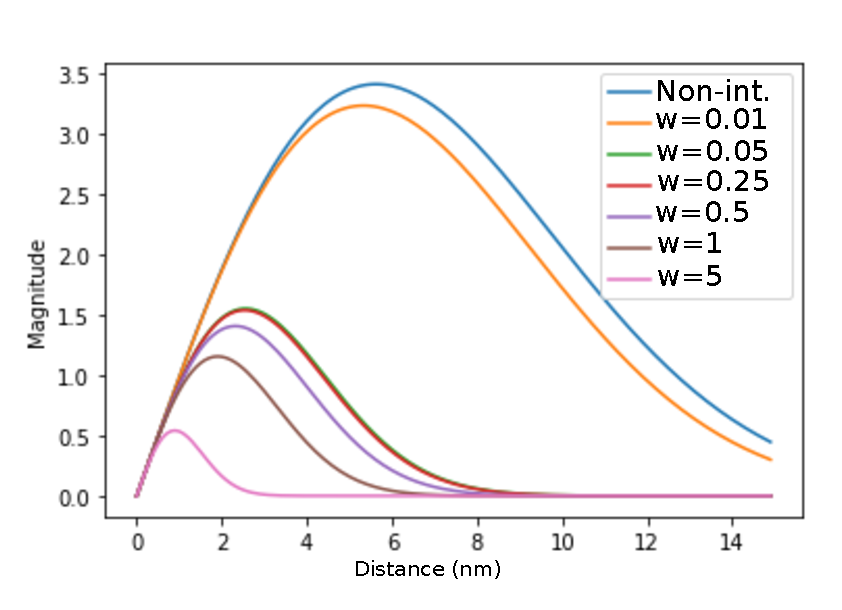
\includegraphics[width=0.5\textwidth]{Graph.eps}
	\caption{A plot of the how the strength constant ($\omega_{r}$) affects the wave function.  The plot is the magnitude of the wave function versus the radial distance between the electrons. }
	\label{fig:graph}
\end{figure}

	
	\subsection{Interacting Case}
	
	We then progressed to the Coulomb interaction case for the Schr$\ddot{\textrm{o}}$dinger equation.  We now find that we can solve for the same Schr$\ddot{\textrm{o}}$dinger equation with a modified potential to account for the Coulomb interactions.  The interaction potential was found to be directly proporational to a coefficienct, $\omega_{r}$, that dictates strength of the oscillator potential.  Using the found energy-eigenvalue relationship, \begin{equation}
	E=\frac{\hbar^{2}}{m\alpha^{2}}\lambda
	\end{equation} where alpha is a fixed constant, we were able to determine the ground state energy for various $\omega_{r}$ (Table \ref{StateTable}).
	
	
	
	\begin{center}
		\begin{tabular}{ccc}
			\hline \hline
			$\omega_{r}$ &  E$_{GS}^{1} (J)$ & E$_{GS}^{2} (J)$ \cite{PhysRevA.48.3561}\\
			\hline
			0.01 & 0.11063 & -- \\
			$^{\star}$0.05 & 0.12310 & 0.1750\\
			$^{\star}$0.25 & 0.53431 & 0.6250\\
			0.5 & 0.54408 & --\\
			1 & 0.96438 & -- \\
			5 & 4.38549 & --\\
			\hline
			\label{StateTable}
		\end{tabular}
		\captionof{table}{Comparison between the ground state energy and $\omega_{r}$. E$_{GS}^{1} (J)$ are ground state energies found in the present work and E$_{GS}^{2} (J)$ are accepted values found in Ref. \cite{PhysRevA.48.3561}.  The $^{\star}$ indicates $\omega_{r}$ values that overlap with the accepted values in Ref. \cite{PhysRevA.48.3561}.  In order to get a good approximation to the accepted value, the ground state energy for $\omega_{r}=0.25$ was found using the second lowest eigenvalue.}
	\end{center}

	Using the general solution of the three dimensional Schr$\ddot{\textrm{o}}$dinger equation from \cite{PhysRevA.48.3561}, we may produce a plot that describes the relationship between the wavefunction, u(r), and the radial distance, r (Figure \ref{fig:graph}).  As the constant ($\omega_{r}$) increases, the magnitude of the wave function decreases.
	
	




\section{Conclusion}

We were able to construct an algorithm that produces the eigenvalues of a tridiagonal matrix that describes the potential of a three dimensional electron-electron interacting Schr$\ddot{\textrm{o}}$dinger equation.  Using units tests and Armadillo functions \cite{Armadillo}, we were able to verify the results of the algorithm.  By timing the algorithm, we were able to see that the Jacobi method produces results in a similar time as the Armadillo equivalent for a small number of meshpoints.  As the number of meshpoints increased, the Jacobi method became much less efficient than the Armadillo equivalent.

The Jacobi rotation algorithm provides one way of finding the eigenvalues for a differential equation.  While it may not be as efficient as other methods, it provides accurate results.


	
	
	
	\bibliography{Project2Bib}
	\bibliographystyle{apsrev4-1}	
	
	
	
\end{document}